\chapter{相对论时空观}
\problem{考虑$2$维欧氏空间, 取一般坐标$\{u,v\}$, 与直角坐标关系为$x = x(u,v)$, $y = y(u,v)$. 求$2$维欧氏空间度规在$\{u,v\}$坐标下的形式.}
\begin{solution}
    由线元的定义, 我们有
    \begin{align*}
        \dd s^2 &= \left(\frac{\pp x}{\pp u} \dd u + \frac{\pp x}{\pp v} \dd v\right)^2 + \left(\frac{\pp y}{\pp u} \dd u + \frac{\pp y}{\pp v} \dd v\right)^2 \\
        &= \left(\frac{\pp x}{\pp u}\right)^2 \dd u^2 + \left(\frac{\pp x}{\pp v}\right)^2 \dd v^2 + \frac{\pp x}{\pp u} \frac{\pp x}{\pp v} \dd u \dd v + \left(\frac{\pp y}{\pp u}\right)^2 \dd u^2 + \left(\frac{\pp y}{\pp v}\right)^2 \dd v^2 + \frac{\pp y}{\pp u} \frac{\pp y}{\pp v} \dd u \dd v \\
        &= \begin{pmatrix}
            \dd u & \dd v
        \end{pmatrix} \begin{pmatrix}
            \left(\frac{\pp x}{\pp u}\right)^2 & \frac{\pp x}{\pp u} \frac{\pp x}{\pp v} \\[0.8em]
            \frac{\pp x}{\pp v} \frac{\pp y}{\pp u} & \left(\frac{\pp y}{\pp v}\right)^2
        \end{pmatrix} \begin{pmatrix}
            \dd u \\ \dd v
        \end{pmatrix}
    \end{align*}
    因此, 度规在$\{u,v\}$坐标下的形式为
    \[
        g_{ij} = \begin{pmatrix}
            \left(\frac{\pp x}{\pp u}\right)^2 & \frac{\pp x}{\pp u} \frac{\pp x}{\pp v} \\[0.8em]
            \frac{\pp x}{\pp v} \frac{\pp y}{\pp u} & \left(\frac{\pp y}{\pp v}\right)^2
        \end{pmatrix}
    \]
\end{solution}

\problem{考虑$3$维欧氏空间, 已知球坐标与直角坐标的关系为$x = r \sin\theta \cos\phi$, $y = r \sin\theta \sin\phi$, $z = r \cos\theta$. 求$3$维欧氏空间度规在球坐标下的形式.}
\begin{solution}
    考虑$3$维欧氏空间中的矢量$\vec{v} = x \h{x} + y \h{y} + z \h{z}$, 由球坐标$\begin{cases}
            x = r \sin\theta \cos\phi \\
            y = r \sin\theta \sin\phi \\
            z = r \cos\theta
        \end{cases}$
    构造坐标系的坐标基矢
    \[
        \begin{aligned}
            \frac{\pp \vec{v}}{\pp r} &= \sin\theta \cos\phi \,\h{x} + \sin\theta \sin\phi \,\h{y} + \cos\theta \,\h{z} \\
            \frac{\pp \vec{v}}{\pp \theta} &= r \cos\theta \cos\phi \,\h{x} + r \cos\theta \sin\phi \,\h{y} - r \sin\theta \,\h{z} \\
            \frac{\pp \vec{v}}{\pp \phi} &= -r \sin\theta \sin\phi \,\h{x} + r \sin\theta \sin\phi \,\h{y}
        \end{aligned}
    \]
    则线元可以写为
    \begin{align*}
        \dd s^2 &= \dd \vec{v} \cdot \dd \vec{v} = g_{ij} \dd u^i \dd u^j\\
        &= \begin{pmatrix}
            \dd r & \dd \theta & \dd \phi
        \end{pmatrix} \begin{pmatrix}
            g_{rr} & g_{r\theta} & g_{\theta\phi} \\
            g_{\theta r} & g_{\theta\theta} & g_{\theta\phi} \\
            g_{\phi r} & g_{\phi\theta} & g_{\phi\phi}
        \end{pmatrix} \begin{pmatrix}
            \dd r \\ \dd \theta \\ \dd \phi
        \end{pmatrix}
    \end{align*}
    其中$g_{ij} = g_{ji} = \frac{\pp \vec{v}}{\pp u^i} \cdot \frac{\pp \vec{v}}{\pp u^j} =
    \frac{\pp x}{\pp u^i} \frac{\pp x}{\pp u^j} + \frac{\pp y}{\pp u^i}
    \frac{\pp y}{\pp u^j} + \frac{\pp z}{\pp u^i} \frac{\pp z}{\pp u^j}$.
    
    \vspace*{1em}
    由于坐标基矢正交, 即非对角元为零, 计算对角元得
    \begin{align*}
        g_{rr} &= \left(\frac{\pp x}{\pp r}\right)^2 + \left(\frac{\pp y}{\pp r}\right)^2 + \left(\frac{\pp z}{\pp r}\right)^2 = (\sin \theta \cos \phi)^2 + (\sin \theta \sin \phi)^2 + (\cos \theta)^2 = 1, \\
        g_{\theta\theta} &= \left(\frac{\pp x}{\pp \theta}\right)^2 + \left(\frac{\pp y}{\pp \theta}\right)^2 + \left(\frac{\pp z}{\pp \theta}\right)^2 = (r \cos \theta \cos \phi)^2 + (r \cos \theta \sin \phi)^2 + (-r \sin \theta)^2 = r^2, \\
        g_{\phi\phi} &= \left(\frac{\pp x}{\pp \phi}\right)^2 + \left(\frac{\pp y}{\pp \phi}\right)^2 + \left(\frac{\pp z}{\pp \phi}\right)^2 = (-r \sin \theta \sin \phi)^2 + (r \sin \theta \cos \phi)^2 = r^2 \sin^2\theta.
    \end{align*}

    将$g_{ij}$代入线元, 得
    \[
        \dd s^2 = \begin{pmatrix}
            \dd r & \dd \theta & \dd \phi
        \end{pmatrix} \begin{pmatrix}
            1 & 0 & 0 \\
            0 & r^2 & 0 \\
            0 & 0 & r^2 \sin^2\theta
        \end{pmatrix} \begin{pmatrix}
            \dd r \\ \dd \theta \\ \dd \phi
        \end{pmatrix}
    \]
    即$3$维欧氏空间度规在球坐标下的形式为
    \[
        g_{ij} = \begin{pmatrix}
            1 & 0 & 0 \\
            0 & r^2 & 0 \\
            0 & 0 & r^2 \sin^2\theta
        \end{pmatrix}
    \]
\end{solution}


\problem{如图\ref{fig:3-3}所示, $2$维环面参数方程为 $\begin{cases}
    x = (R + r \cos \theta) \cos \phi, \\
    y = (R + r \cos \theta) \sin \phi, \\
    z = r \sin \theta
\end{cases}$, 其中 $R$ 和 $r$ 是常数, $\{\theta, \phi\}$ 为环面的坐标, 取值为 $0$ 到 $2\pi$. 求$2$维环面的度规.}
\begin{figure}[h]
    \centering
    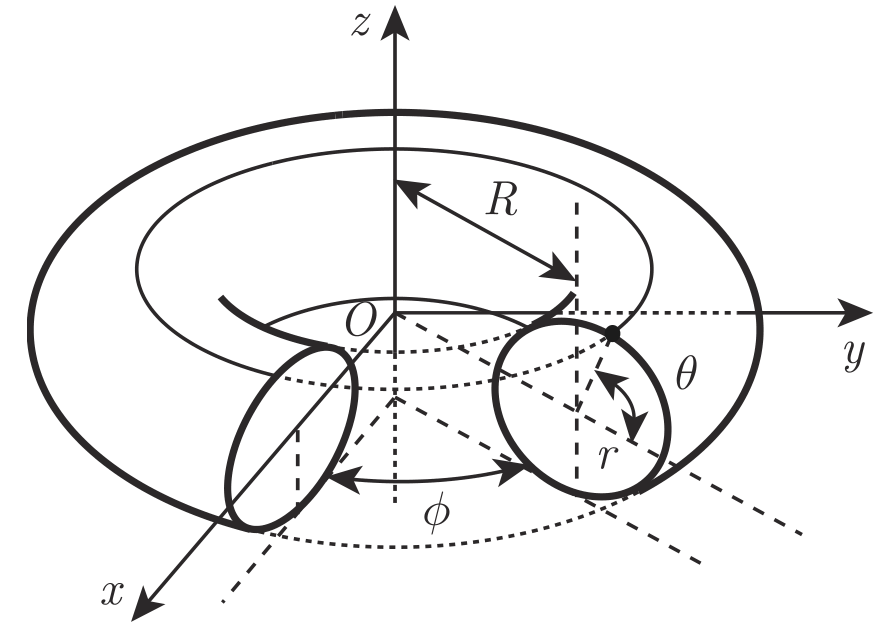
\includegraphics[width=0.3\textwidth]{content/Figures/3-3}
    \caption{ }
    \label{fig:3-3}
\end{figure}

